
\chapter{Compressing Ping6}

\section{Introduction}

In this chapter, we are going to setup the compression of a ping6 request. An ICMPv6 request is composed of an IPv6 header, followed by a \Index{ICMPv6 request} message.

\begin{termc}[backgroundcolor=\color{gray!10}, basicstyle=\ttfamily\tiny, escapechar=@]
Internet Protocol Version 6, Src: 2a01:cb08:903a:bd00:a8c4:5c6d:c2b5:84be, Dst: 
2001:470:1f21:1d2::1
    0110 .... = Version: 6
    .... 0000 0000 .... .... .... .... .... = Traffic Class: 0x00 (DSCP: CS0, ECN: Not-ECT)
        .... 0000 00.. .... .... .... .... .... = Differentiated Services Codepoint: Default (0)
        .... .... ..00 .... .... .... .... .... = Explicit Congestion Notification: Not ECN-Capable Transport (0)
    .... .... .... 1000 0000 1000 0000 0000 = Flow Label: 0x80800
    Payload Length: 16
    Next Header: ICMPv6 (58)
    Hop Limit: 56
    Source: 2a01:cb08:903a:bd00:a8c4:5c6d:c2b5:84be
    Destination: 2001:470:1f21:1d2::1
    
Internet Control Message Protocol v6
    Type: Echo (ping) request (128)
    Code: 0
    Checksum: 0x3982 [correct]
    [Checksum Status: Good]
    Identifier: 0x70ef
    Sequence: 699

    Data (8 bytes)
        Data: 609ab0db000aecb7
        [Length: 8]

0000  60 08 08 00 00 10 3a 38 2a 01 cb 08 90 3a bd 00   `.....:8*....:..
0010  a8 c4 5c 6d c2 b5 84 be 20 01 04 70 1f 21 01 d2   ..\m.... ..p.!..
0020  00 00 00 00 00 00 00 01 80 00 39 82 70 ef 02 bb   ..........9.p...
0030  60 9a b0 db 00 0a ec b7  
\end{termc}

The following compression rule can be applied to that traffic.

\begin{lstlisting}[basicstyle=\ttfamily\tiny, caption={rule 6/3 for ping traffic}, caption=fig-rule-ping, backgroundcolor=\color{yellow}]

{
    "DeviceID" : "udp:83.199.24.39:8888",
    "SoR" : [
	{
	    "RuleID": 6,
	    "RuleIDLength": 3,
	    "Compression": [
		{"FID": "IPV6.VER", "TV": 6, "MO": "equal", "CDA": "not-sent"},
		{"FID": "IPV6.TC",  "TV": 0, "MO": "equal", "CDA": "not-sent"},
		{"FID": "IPV6.FL",  "TV": 0, "MO": "ignore","CDA": "not-sent"},
		{"FID": "IPV6.LEN",          "MO": "ignore","CDA": "compute-length"},
		{"FID": "IPV6.NXT", "TV": 58, "MO": "equal", "CDA": "not-sent"},
		{"FID": "IPV6.HOP_LMT", "TV" : 64,"MO": "ignore","CDA": "not-sent"},
		{"FID": "IPV6.DEV_PREFIX","TV": "2001:470:1F21:1D2::/64",
                                               "MO": "equal","CDA": "not-sent"},
		{"FID": "IPV6.DEV_IID", "TV": "::1","MO": "equal","CDA": "not-sent"},
		{"FID": "IPV6.APP_PREFIX",         "MO": "ignore","CDA": "value-sent"},
		{"FID": "IPV6.APP_IID",         "MO": "ignore","CDA": "value-sent"},
		{"FID": "ICMPV6.TYPE",  "DI": "DW", "TV": 128,"MO": "equal","CDA": "not-sent"},
		{"FID": "ICMPV6.TYPE",  "DI": "UP", "TV": 129,"MO": "equal","CDA": "not-sent"},
		{"FID": "ICMPV6.CODE",  "TV": 0,  "MO": "equal","CDA": "not-sent"},
		{"FID": "ICMPV6.CKSUM", "TV": 0, "MO": "ignore","CDA": "compute-checksum"},
		{"FID": "ICMPV6.IDENT", "TV": 0,"MO": "ignore","CDA": "value-sent"},
		{"FID": "ICMPV6.SEQNO", "TV": 0,"MO": "ignore","CDA": "value-sent"}
		
	       ]
	} ] }
	
\end{lstlisting}



\section{Understanding compression rules}

A rule contains a list of fields description:
\begin{itemize}
    \item starting with a \Index{Field ID}. openSCHC uses a string structured with the protocol name (\texttt{IPV6} and \texttt{ICMPV6} in the rule above). Field ID uses keyword \texttt{\Index{FID}}.

    \item A \Index{Target Value} (\texttt{TV}) may be present and contains the value the rule expected to find in the field.

    \item A \Index{Direction Indicator} (\texttt{DI}) can be associated to a field. In the above example, \Indexr{\texttt{ICMPV6.TYPE}} is repeated twice for uplink and downlink. When the direction is not specified, openSCHC considers the field as bi-directionnal.

    \item A \Index{Matching Operator} (\texttt{MO}) specifies the comparison between the target Value  (\texttt{TV}) and the Field Value (\texttt{FV}) present in the packet to be compressed. \rfc{8724} defines 4 MO:

    \begin{itemize}
    \item \texttt{\Index{ignore}}: the FV is ignored therefore, the result of the field comparison is always true.
    \item \texttt{\Index{equal}}: the result of the comparison is true is the value contained in the \texttt{TV} is equal to the value contained if the \texttt{FV}. OpenSCHC allows integer and strings for the comparison.
    \item \texttt{\Index{MSB}}: is true only if the first bits of the \texttt{TV} are equal to the first bits of the \texttt{FV}. The comparison length in bits is specified in the rule with the keywork \texttt{MO.val}. For string comparison, openSCHC impose a  multiple of 8 bits for the length.
    \item \texttt{\Index{match-mapping}}: The \texttt{TV} contains an array of values. The comparison is true, if the \texttt{FV} appears somewhere in the list.
    \end{itemize}

    A rule is selected if all the comparison are true and the packet contains no other fields. 


    \item When a rule is selected, the \Index{Compression Decompression Actions} (\texttt{CDA}) are applied to the packet fields. \rfc{8724} defines several CDAs, among them:

    \begin{itemize}
        \item \Indexs{\texttt{not-sent}}: the \texttt{FV} is not sent, the decompressor will use the value stored in the rule to recover the value\marge{not-sent}.
        \item \Index{\texttt{value-sent}}: the value is explicitely sent as a residue. The decompressor will use the residue to recover the value.
        \item \Index{\texttt{LSB}}: the least significant bits are sent as residue. The decompressor will combine the \texttt{TV} and the residue to recover the field. LSB can only be used with a MSB MO. No argument are needed for LSB. The LSB size is defined from the field size and the MSB size.
        \item \Index{\texttt{mapping-sent}} : the index in the array is sent as residue. The decompressor will use the idenx to recover the value. This CDA can only be used with a match-mapping MO.
        \item \Index{\texttt{compute-*}}: the \texttt{FV} is not sent, the decompressor will use a specific algorithm to recover the value, such as compute the length or compute a checksum.
    \end{itemize}

\end{itemize}

\section{Compressing an ICMPv6 echo request packet}

In the above example, the \Indexr{\texttt{IPV6.VERSION}} field is not sent, the value 6 is stored is the rule. 
The \Indexr{\texttt{IPV6.NXT}} follows the same behavior, since ICMPv6 is expected, the \texttt{TV} is 58.

~

Note that \Indexr{\texttt{IPV6.FL}} and \Indexr{\texttt{IPV6.HOP\_LMT}}[0.45cm] use the \Indexs{ignore}/\Indexs{not-sent}\marge{ignore/not-sent} combination. During the rule selection, the \texttt{FL} is not taken into account, but during decompression the value stored in the rule is used. The reason is that IPv6 Flow Label (\texttt{IPV6.FL}) can be different from 0, in the capture the value is \texttt{0x80800}. 

~

For IPv6 Hop Limit  (\Indexr{\texttt{IPV6.HOP\_LMT}}) the value cannot be forecast, depends of how many routers are crossed and may vary during from one packet to the other. The rule ignores the value and generate a hop limit of 64. To be valid, this implies that the device will not forward anymore the packet. If the device acts as a router the Hop Limit field must be sent.

~

The address fields compression is more interesting, there is not source or destination address in the SCHC rule. SCHC defines the device  and the application \Index{addresses}\footnote{This will apply also for UDP port number}. The rule becomes independent of the direction. OpenSCHC splits the addresses into a 64 bit long prefix and a 64 bit long \Index{IID}. 

In our scenario the device address is not sent, since the value is known by the device. On the opposite, we allow any host to ping the device\footnote{This behavior has to be prohibited in a LPWAN network, for security reasons, since in this scenario we are using an UDP tunnel, there is no security issue.}. The destination address is fully sent to the device.

~~

At the ICMPv6 level, the type field is elided regarding the direction. The Echo value (128) is expected downlink; form the application to the device, and the Echo reply (129) on the other direction. In both cases the ICMPv6 code is expected to be 0.

~~~

The identifier (\Indexr{\texttt{ICMPv6.IDENT}}) and sequence number (\Indexr{\texttt{ICMPV6.SEQNO}}[0.45cm]) are not compressed and send as residue.

~~

The other fields \Indexr{\texttt{IPV6.LENGTH}} and \Indexr{\texttt{ICMPV6.CHECKSUM}}[0.45cm] are not sent and computed by the other side.

~~

The SCHC packet has the following format:

\begin{figure}[!ht] 
\centering 
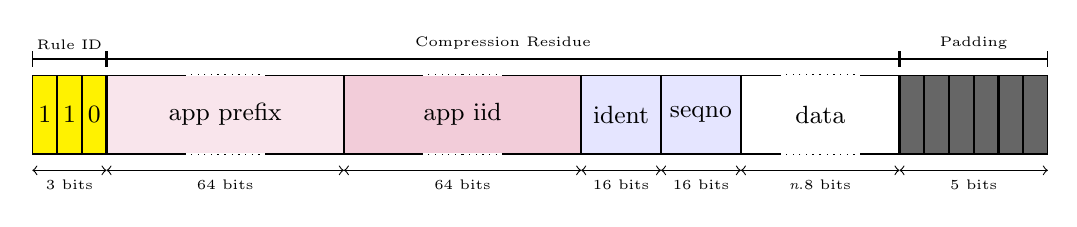
\begin{tikzpicture}

\draw (0,0) node (b1)  [rectangle, draw, minimum height=1cm, minimum width = 0.3cm, fill=yellow] {};
\draw(b1) node {\small{1}};
\draw (b1.east) node (b2)  [right, rectangle, draw, minimum height=1cm, minimum width = 0.3cm, fill=yellow] {};
\draw(b2) node {\small{1}};
\draw (b2.east) node (b3)  [right,rectangle, draw, minimum height=1cm, minimum width = 0.3cm, fill=yellow] {};
\draw(b3) node {\small{0}};

\path(b1.north) -- +(0, 0.2) coordinate(hlineu);

\draw [|-|] (b1.west |- hlineu) -- coordinate(a) (b3.east |- hlineu) ;
\draw (a) node [above] {\tiny{Rule ID}};

\path(b1.south) -- +(0, -0.2) coordinate(hline);

\draw [<->] (b1.west |- hline) -- coordinate(a) (b3.east |- hline) ;
\draw (a) node [below] {\tiny{3 bits}};


\draw (b3.east) node (pref) [right, rectangle, draw, minimum height=1cm, minimum width=3cm, fill=purple!10]{};

\draw [white, thick] (pref.north) -- +(0.5, 0);
\draw [white, thick] (pref.north) -- +(-0.5, 0);
\draw [dotted] (pref.north) -- +(0.5, 0);
\draw [dotted] (pref.north) -- +(-0.5, 0);

\draw [white, thick] (pref.south) -- +(0.5, 0);
\draw [white, thick] (pref.south) -- +(-0.5, 0);
\draw [dotted] (pref.south) -- +(0.5, 0);
\draw [dotted] (pref.south) -- +(-0.5, 0);

\draw (pref) node {\small{app prefix}};

\path(b1.south) -- +(0, -0.2) coordinate(hline);


\draw (pref.east) node (iid) [right, rectangle, draw, minimum height=1cm, minimum width=3cm, fill=purple!20]{};

\draw [white, thick] (iid.north) -- +(0.5, 0);
\draw [white, thick] (iid.north) -- +(-0.5, 0);
\draw [dotted] (iid.north) -- +(0.5, 0);
\draw [dotted] (iid.north) -- +(-0.5, 0);

\draw [white, thick] (iid.south) -- +(0.5, 0);
\draw [white, thick] (iid.south) -- +(-0.5, 0);
\draw [dotted] (iid.south) -- +(0.5, 0);
\draw [dotted] (iid.south) -- +(-0.5, 0);

\draw (iid) node {\small{app iid}};

\path(b1.south) -- +(0, -0.2) coordinate(hline);

\draw [<->] (pref.west |- hline) -- coordinate(a) (pref.east |- hline) ;
\draw (a) node [below] {\tiny{64 bits}};

\draw [<->] (iid.west |- hline) -- coordinate(a) (iid.east |- hline) ;
\draw (a) node [below] {\tiny{64 bits}};

\draw (iid.east) node (ident) [right, rectangle, draw, minimum height=1cm, minimum width=1cm, fill=blue!10]{};
\draw (ident.text) node {\small{ident}};

\draw [<->] (ident.west |- hline) -- coordinate(a) (ident.east |- hline) ;
\draw (a) node [below] {\tiny{16 bits}};

\draw (ident.east) node (seqno) [right, rectangle, draw, minimum height=1cm, minimum width=1cm, fill=blue!10]{};
\draw (seqno.text) node {\small{seqno}};

\draw [<->] (seqno.west |- hline) -- coordinate(a) (seqno.east |- hline) ;
\draw (a) node [below] {\tiny{16 bits}};

\draw (seqno.east) node (data) [right, rectangle, draw, minimum height=1cm, minimum width=2cm]{};
\draw (data.text) node {\small{data}};

\draw [white, thick] (data.north) -- +(0.5, 0);
\draw [white, thick] (data.north) -- +(-0.5, 0);
\draw [dotted] (data.north) -- +(0.5, 0);
\draw [dotted] (data.north) -- +(-0.5, 0);

\draw [white, thick] (data.south) -- +(0.5, 0);
\draw [white, thick] (data.south) -- +(-0.5, 0);
\draw [dotted] (data.south) -- +(0.5, 0);
\draw [dotted] (data.south) -- +(-0.5, 0);

\draw [<->] (data.west |- hline) -- coordinate(a) (data.east |- hline) ;
\draw (a) node [below] {\tiny{\textit{n}.8 bits}};

\draw (data.east) node (p1)  [right, rectangle, draw, minimum height=1cm, minimum width = 0.3cm, fill=black!60] {};
\draw (p1.east) node (p2)  [right, rectangle, draw, minimum height=1cm, minimum width = 0.3cm, fill=black!60] {};
\draw (p2.east) node (p3)  [right,rectangle, draw, minimum height=1cm, minimum width = 0.3cm, fill=black!60] {};
\draw (p3.east) node (p4)  [right,rectangle, draw, minimum height=1cm, minimum width = 0.3cm, fill=black!60] {};
\draw (p4.east) node (p5)  [right,rectangle, draw, minimum height=1cm, minimum width = 0.3cm, fill=black!60] {};
\draw (p5.east) node (p6)  [right,rectangle, draw, minimum height=1cm, minimum width = 0.3cm, fill=black!60] {};

\draw [|-|] (p1.west |- hlineu) -- coordinate(a) (p6.east |- hlineu) ;
\draw (a) node [above] {\tiny{Padding}};

\draw [<->] (p1.west |- hline) -- coordinate(a) (p6.east |- hline) ;
\draw (a) node [below] {\tiny{5 bits}};

\draw [|-|] (b3.east |- hlineu) -- coordinate(a) (p1.west |- hlineu) ;
\draw (a) node [above] {\tiny{Compression Residue}};


\end{tikzpicture}
\caption{ICMPv6 Compression Residue} 
\label{fig-residue} 
\end{figure} 

The rule ID takes 3 bits, followed by the compression \Index{residue}s, the ICMPv6 payload and some padding bits. Since the Rule ID length is 3 bit long and the rest is byte aligned, 5 bits are needed to align the SCHC packet on a  L2-word (i.e. 1 byte).

\section {Compression process}

In OpenSCHC, SCHC Compresssion/Decompression (CD) and Frgamentation/Reassembly (FR) processes are done by the SCHC Machine.

\begin{figure}[!ht] 
\centering 


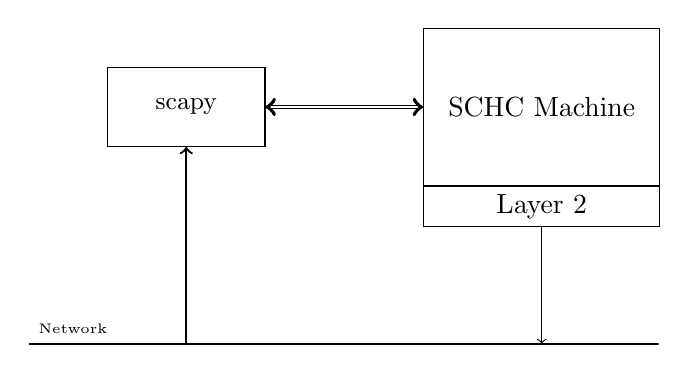
\begin{tikzpicture}

\draw (0,0) node (scapy) [rectangle, draw, minimum width=2cm, minimum height=1cm] {};

\draw (scapy) node {\small{scapy}};

\draw [<-] [thick] (scapy.south) -- coordinate(d) +(0, -2.5) coordinate (a);
\draw [thick] (a) -- +(6, 0) -- +(-2, 0) coordinate (b);

\draw(b) node [above right] {\tiny{Network}};

\draw [<->, double] (scapy.east) -- +(2, 0) coordinate (c);

\draw (c) node (SCHC) [right, rectangle, draw, minimum width=3cm, minimum height=2cm] {};
\draw (SCHC) node {SCHC Machine};
\draw (SCHC.south) node (L2)  [below, rectangle, draw, minimum width = 3cm, minimum height=0.5cm] {};
\draw (L2) node {Layer 2};

\draw [->] (L2.south) -- (L2.south |-a);


\end{tikzpicture}

\caption{Ping gateway architecture} 
\label{fig-schc-archi} 
\end{figure} 

Figure~\vref{fig-schc-archi} gives the architecture of the ping gateway. 
\Index{Scapy} \textit{sniff} function gets traffic on the network. 
This traffic is composed of IPv6 packets that could be compressed and tunneled SCHC packets that are decompressed. 



\subsection{The code}
\label{sec-compr_code}


The scapy module calls the SCHC Machine, in charge of CD-FR processes. Layer 2 allows to send decompressed packet or a SCHC packet on the network. 

\subsubsection{Main program}

\pythonlst[firstline=1,lastline=15, firstnumber=1]{ping_core1.py}


This program~\pprog{ping\_core1.py} shows how to compress ICMPv6 packets and send them on a UDP tunnel to a device. It starts with the modules importation from scapy, openSCHC and some regular python modules. Note the importation of the \Index{\texttt{scapy\_connection}} module, located on the working directory. This module implements the scheduler and the methods to send packets.

\pythonnxt[firstline=18,lastline=22, firstnumber=18]{ping_core1.py}

The compression process starts with the creation of a Rule Manager \texttt{rm} to include the rules from file \texttt{icmp.json} (cf. Listing~\vref{rule-icmp1}), which contains  the compression rules we saw below and a NoAck fragmentation rule.


\begin{lstlisting}[caption={rule icmp1.json}, backgroundcolor=\color{yellow}, label=rule-icmp1, basicstyle=\ttfamily\tiny],
{
    "DeviceID" : "udp:83.199.24.39:8888",
    "SoR" : [
	 {
	    "RuleID": 6,
	    "RuleIDLength": 3,
	    "Compression": [
		{"FID": "IPV6.VER", "TV": 6, "MO": "equal", "CDA": "not-sent"},
		{"FID": "IPV6.TC",  "TV": 0, "MO": "equal", "CDA": "not-sent"},
		{"FID": "IPV6.FL",  "TV": 0, "MO": "ignore","CDA": "not-sent"},
		{"FID": "IPV6.LEN",          "MO": "ignore","CDA": "compute-length"},
		{"FID": "IPV6.NXT", "TV": 58, "MO": "equal", "CDA": "not-sent"},
		{"FID": "IPV6.HOP_LMT", "TV" : 255,"MO": "ignore","CDA": "not-sent"},
		{"FID": "IPV6.DEV_PREFIX","TV": "2001:470:1F21:1D2::/64",
                                               "MO": "equal","CDA": "not-sent"},
		{"FID": "IPV6.DEV_IID", "TV": "::1","MO": "equal","CDA": "not-sent"},
		{"FID": "IPV6.APP_PREFIX",         "MO": "ignore","CDA": "value-sent"},
		{"FID": "IPV6.APP_IID",         "MO": "ignore","CDA": "value-sent"},
		{"FID": "ICMPV6.TYPE",  "DI": "DW", "TV": 128,"MO": "equal","CDA": "not-sent"},
		{"FID": "ICMPV6.TYPE",  "DI": "UP", "TV": 129,"MO": "equal","CDA": "not-sent"},
		{"FID": "ICMPV6.CODE",  "TV": 0,  "MO": "equal","CDA": "not-sent"},
		{"FID": "ICMPV6.CKSUM", "TV": 0, "MO": "ignore","CDA": "compute-checksum"},
		{"FID": "ICMPV6.IDENT", "TV": 0,"MO": "ignore","CDA": "value-sent"},
		{"FID": "ICMPV6.SEQNO", "TV": 0,"MO": "ignore","CDA": "value-sent"}
		
	    ]
	 },{
		"RuleID" : 12,
		"RuleIDLength" : 11,
		"Fragmentation" : {
			"FRMode": "NoAck",
			"FRDirection": "DW"
		}
	} 
    ]
  }
\end{lstlisting}

This rule must be adapted to your environment. The \texttt{DeviceID} must reflect the IPv4 public address of your device and the Target Value of \Indexr{\texttt{IPV6.DEV\_PREFIX}} must be set to a IPv6 prefix of your domain, such as the ones allocated by Hurricane Electric.

\pythonnxt[firstline=48,lastline=57, firstnumber=48]{ping_core1.py}

The position of the SCHC instance has to be specified. In our example, we define our role as a core. Then, we create the UDP tunnel to receive SCHC packets from devices. The default port number is \texttt{0x5C4C}.

A \texttt{lower\_layer} is created to be used by the SCHC machine when SCHC packet will have to be sent, and a \texttt{system} is created to manage events. The latter includes a \Index{scheduler}.  Both are defined in the \Index{\texttt{scapy\_connection}} module. 


From that \texttt{system} a reference to the \texttt{scheduler} is extracted to be used in the \texttt{processPkt} function as a global variable.

\pythonnxt[firstline=58,lastline=63, firstnumber=58]{ping_core1.py}

The previously created classes are regrouped arounf a \Index{SCHC machine} which will process packets for compression and fragmentation. A \texttt{schc\_machine} instance is created and the previously created rule manager is associated to it.

\pythonnxt[firstline=65,lastline=65, firstnumber=65]{ping_core1.py}


Finally, the scapy \texttt{sniff} function is called. This last line never returns. The \texttt{processPkt} function is called each time a packet is received on interface \texttt{ens3}\footnote{Scapy allowed to listen simultaneously to several interfaced, for example \texttt{["ens3", "he-ipv6"]}, but since this feature returns sometime some errors, we prefer to listen only to interface \texttt{"ens3"} which will carried tunneled IPv6 packets from Hurricane Electrics.}.

\subsubsection{Frame processing}

\pythonnxt[firstline=24,lastline=29, firstnumber=24]{ping_core1.py}

The \texttt{processPkt} function starts by calling the SCHC machine through the \pfunction{scapy\_scheduler}{run} method. This function must be called regularly, which is the case when some traffic occurs in the network, so it is important not to filter too much incoming traffic.

~

The functions looks for two types of packets:
\begin{itemize}
    \item SCHC tunneled packets coming from devices to the UDP port we defined (\texttt{0x5C4C} in our case),
    \item IPv6 tunneled packets from Hurricane Electric easily recognisable through the use of IP proto 41.
\end{itemize}

\pythonnxt[firstline=31,lastline=44, firstnumber=31]{ping_core1.py}

First, a test done to ensure that the frame has an Ethernet encapsulation\footnote{That wouldbe the case, if the Hurrican Electric interface was directly listened by scapy.}. Then we filter the frames to keep only those with:
\begin{itemize}
    \item an Ethertype equal to 0x800 indicating an IPv4 packet,
    \item an IPv4 protocol number equal to 17 indicating an UDP message,
    \item and a destination port of \texttt{0x5C4C} indicating a SCHC packet.
\end{itemize}

If all these conditions are met, we are sure that the socket has received a packet. We read the socket and get the message (\texttt{schc\_pkt}) and the device address (\texttt{addr}) which send the SCHC packet. 

~

The next step is to build the \Index{DeviceID} (\texttt{other\_end}) by concatenating the \texttt{udp} keyword, followed with the sender IPv4 address and its port number. The DeviceID must match the one stored in the rule (cf. Listing~\vref{rule-icmp1}).

~~

Once the SCHC packet and its device ID are known, the \pfunction{SCHCProtocol}{schc\_recv} method is called. This method looks the the rule ID, the associated rule and apply it. If it is a compression rule, it will returns the uncompressed packet. 

\pythonnxt[firstline=45,lastline=46, firstnumber=45]{ping_core1.py}

If the IP protocol value is 41, then we have a tunneled IPv6 packet over IPv4. The first 34 bytes corresponding to the Ethernet and IPv4 headers are removed, and the resulting IPv6 packet is send to the SCHC machine for compression. The SCHC packet will be sent using \Index{\texttt{scapy\_connection}} functions.

\subsection{The execution}

Start the program, in sudo mode:

\begin{termc}[backgroundcolor=\color{palerod}, basicstyle=\ttfamily\small, escapechar=@]
$ sudo python3.9 ping_core1.py 
\end{termc}

The program will display the rules and cursor spins, indicating the SCHC machine is running\footnote{The number of received packets determines the spinning speed. It takes 10 packets to change the cursor appearance.}. 

Start pinging the device, from any host in the Internet with IPv6 connectivity. to the IPv6 address of the device defined in the rule, the \texttt{-c 1} limits the number of ping messages. 

\begin{termc}[backgroundcolor=\color{pink!20}, basicstyle=\ttfamily\small, escapechar=@]
$ ping6 2001:470:1f21:1d2::1 -c 1
\end{termc}

Of course there is no answer to the ping, the openSCHC core instance displays some messages. They can be avoided, if the \texttt{verbose} argument is set to False or not specified when creating the \texttt{schc\_machine} object. 

\begin{termc}[backgroundcolor=\color{palerod}, basicstyle=\ttfamily\tiny, escapechar=@]
schc recv-from-l3 None None b'`\x05\x0c\x00\x00\x10:8*\x01\xcb\x08\x90:\xbd\x00I\xe0\xa3\xec\x01Vv\x9c \x01\x04p...'
schc parser {('IPV6.VER', 1): [6, 4], ('IPV6.TC', 1): [0, 8], ('IPV6.FL', 1): [330752, 20]...} 
schc compression rule {'RuleID': 6, 'RuleIDLength': 3, 'Compression': [{'FID': 'IPV6.VER', 'FL': 4, ...}
schc compression result b'\xc5\x40\x39\x61\x12\x07\x57\xa0\x09\x3c\x14\x7d\x80\x2a\xce...'/227
schc fragmentation not needed size=227
\end{termc}
 
This trace gives the openSCHC compression process divided into several steps:
\begin{itemize}
\item Parse the packet; from a sequence of byte received on the network, create a list of fields containing the field identification and their associated value.
\item Find a valid compression rule; ask the rule manager to find a rule matching the parsed packet. The rule selection will also provide the device ID.
\item Apply the compression rule.
\item Send the SCHC packet to the device ID.
\end{itemize}

~~ 

In more details:
\begin{itemize}
    \item The first line (\texttt{recv-from-l3}) dumps the original IPv6 packet received by the compressor, corresponding in hexadecimal to:
\end{itemize}

\begin{termc}[backgroundcolor=\color{palerod}, basicstyle=\ttfamily\tiny, escapechar=@]
60050c0000103a382a01cb08903abd0049e0a3ec0156769c200104701f2101d20000000000000001800051fb48b20000609f882600060ed2
\end{termc}

\begin{itemize}
    \item The second line (\texttt{parser}) shows three elements returned by the parser. The first one is the list of fields, the second one is the data following the list of fields and the third one is a status code. The parsed headers are displayed figure~\ref{list-parsed-icmpv6}:
\end{itemize}

\begin{termc}[backgroundcolor=\color{palerod}, basicstyle=\ttfamily\small, escapechar=@, label=list-parsed-icmpv6, caption={Parsed IPv6/ICMPv6 header fields}]
{('ICMPV6.CKSUM', 1): [20987, 16],
 ('ICMPV6.CODE', 1): [0, 8],
 ('ICMPV6.IDENT', 1): [18610, 16],
 ('ICMPV6.SEQNO', 1): [0, 16],
 ('ICMPV6.TYPE', 1): [128, 8],
 ('IPV6.APP_IID', 1): [b'I\xe0\xa3\xec\x01Vv\x9c', 64],
 ('IPV6.APP_PREFIX', 1): [b'*\x01\xcb\x08\x90:\xbd\x00', 64],
 ('IPV6.DEV_IID', 1): [b'\x00\x00\x00\x00\x00\x00\x00\x01', 64],
 ('IPV6.DEV_PREFIX', 1): [b' \x01\x04p\x1f!\x01\xd2', 64],
 ('IPV6.FL', 1): [330752, 20],
 ('IPV6.HOP_LMT', 1): [56, 8, 'fixed'],
 ('IPV6.LEN', 1): [16, 16, 'fixed'],
 ('IPV6.NXT', 1): [58, 8, 'fixed'],
 ('IPV6.TC', 1): [0, 8],
 ('IPV6.VER', 1): [6, 4]}
\end{termc}
\begin{itemize}

As shown in figure~\vref{list-parsed-icmpv6}, a header description is a dictionnary where keys are tuple Field ID and position\footnote{In this example, position is always 1 since no field is repeated several time.}, and the value is the tuple containing field value and field size in bits.
\end{itemize}

\begin{itemize}
 The next return element is the data, i.e. the bytes following the parsed header:
\end{itemize}

\begin{termc}[backgroundcolor=\color{palerod}, basicstyle=\ttfamily\small, escapechar=@]
b'`\x9f\x88&\x00\x06\x0e\xd2'
\end{termc}
\begin{itemize}
and the error code is None since the parser recognize all the fields.
\end{itemize}

\begin{itemize}
This no surprise, the rule 6/3 matches. 
\end{itemize}


\begin{itemize}

\item The third line \texttt{compression result} gives the SCHC packet. Note the \texttt{/227}\footnote {227 \% 8 = 3.  Since the all the residues are byte alligned, the 3 represent the rule ID length. 5 bits of padding will have to be addeed.} at the end, indicating the length in bits. Converted in hexadecimal, we have:
\end{itemize}


\begin{termc}[backgroundcolor=\color{palerod}, basicstyle=\ttfamily\small, escapechar=@]
b'c5403961120757a0093c147d802aced3891640000c13f104c000c1da40'
\end{termc}


\begin{itemize}
    \item Finally, no fragmentation is required, so the SCHC packet is directly sent on the tunnel. A frame capture of UDP frame with port 0x5C4C gives:
\end{itemize}



\begin{termc}[backgroundcolor=\color{palerod}, basicstyle=\ttfamily\footnotesize]
>sudo tcpdump -nXi ens3 udp port 0x5C4C
tcpdump: verbose output suppressed, use -v or -vv for full protocol decode
listening on ens3, link-type EN10MB (Ethernet), capture size 262144 bytes
16:41:48.609729 IP 51.91.121.182.23628 > 83.199.24.39.8888: UDP, length 29
	0x0000:  4500 0039 ac95 4000 4011 751f 335b 79b6  E..9..@.@.u.3[y.
	0x0010:  53c7 1827 5c4c 22b8 0025 1936[c540 3961  S..'\L"..%.6.@9a
	0x0020:  1207 57a0 093c 147d 802a ced3 8e5f c000  ..W..<.}.*..._..
	0x0030:  0c13 fbb5 8000 d951 80]                   .......Q.

\end{termc}

\section{The Decompression Process}

 Now that we send SCHC packet to the device, lets process the SCHC packet on this side.
 
\subsection{Decompression}

Let's do the same operation on the device side. The code is almost the same, as the core SCHC. It is important to note that the rules are excactly the same as the one we used in the core SCHC.

\pycomlst[firstline=46,lastline=57, firstnumber=46]{ping_device1.py}

The position is changed to \texttt{T\_POSITION\_DEVICE}.  Since the \texttt{device\_id}, in our example, is based on a public IP address, the call to \texttt{https://api.ipify.org} returns the IPv4 public address of the device. We create a UDP socket for port 8888.


\pycomnxt[firstline=59,lastline=69, firstnumber=59]{ping_device1.py}

The \texttt{lower\_layer}, \texttt{system} and \texttt{schc\_machine} are declared the same way as in the core SCHC.  The interface name is adapted to its name on the device side.

\pycomnxt[firstline=35,lastline=43, firstnumber=35]{ping_device1.py}

We go a little bit further in the processing 
If in the packet processing, a tunnel is identified. Even, if the scapy buffer, constains the packet, the regular \texttt{recvfrom} socket function is used to recover the data. They are sent to the SCHC machine, which decompress it and returns a field description.

\begin{lstlisting}
{('ICMPV6.CKSUM', 1): ('CCCC', 16),
 ('ICMPV6.CODE', 1): [0, 8],
 ('ICMPV6.IDENT', 1): [31025, 16],
 ('ICMPV6.SEQNO', 1): [8749, 16],
 ('ICMPV6.TYPE', 1): [128, 8],
 ('IPV6.APP_IID', 1): [5323434993581979292, 64],
 ('IPV6.APP_PREFIX', 1): [3026923662209629440, 64],
 ('IPV6.DEV_IID', 1): [b'\x00\x00\x00\x00\x00\x00\x00\x01', 64],
 ('IPV6.DEV_PREFIX', 1): [b' \x01\x04p\x1f!\x01\xd2', 64],
 ('IPV6.FL', 1): [0, 20],
 ('IPV6.HOP_LMT', 1): [255, 8],
 ('IPV6.LEN', 1): ('LLLL', 16),
 ('IPV6.NXT', 1): [58, 8],
 ('IPV6.TC', 1): [0, 8],
 ('IPV6.VER', 1): [6, 4]}
\end{lstlisting}

Note that \texttt{IPV6.LEN} and \texttt{ICMPV6.CKSUM} to, which a \texttt{compute-*} CDA had been associated, contain respectively \texttt{'LLLL'} and \texttt{'CCCC'} values\footnote{In fact, these values will be computed directly by scapy when generating a packet from this field description.}.

\subsection{Device optimization}

In the previous example (cf. listing~\vref{prog-ping-device1}) we started to reconstruct the packet. We can optimize the process on the device. The rule 6/3 (cf. rule figure~\vref{rule-icmp1}) has been associated to the ping traffic. For the downlink, the type is an Echo Request (128) and for the uplink the type is an Echo Reply (129). The other fields remain unchanged in both directions.


~~

Therefore, when the device receives an SCHC packet with rule 6/3, it can send it back to the SCHC core instance to answer with a reply.
We simplify the ping request processing by testing if the rule ID is equal\footnote{Remeber the comparison must be done on the rule ID value and length}.. to the pink6 rule. In that case, the device just echoes the SCHC packet containing the sequence number and identifier, as show in listing figure~\vref{prog-ping-device2}.

\begin{lstlisting}[language=Python, caption={Program ping\_device2.py}, label=prog-ping-device2, basicstyle=\ttfamily\scriptsize]
import sys
# insert at 1, 0 is the script path (or '' in REPL)
sys.path.insert(1, '../../src/')

from scapy.all import *

import gen_rulemanager as RM
from protocol import SCHCProtocol
from scapy_connection import *
from gen_utils import dprint, sanitize_value
from gen_bitarray import *

import pprint
import binascii
import socket
import ipaddress

# Create a Rule Manager and upload the rules.
rm = RM.RuleManager()
rm.Add(file="icmp1.json")
rm.Print()

def processPkt(pkt):
    """ called when scapy receives a packet, since this function takes only one argument,
    schc_machine and scheduler must be specified as a global variable.
    """

    scheduler.run(session=schc_machine)

    # look for a tunneled SCHC pkt
    if pkt.getlayer(Ether) != None: #HE tunnel do not have Ethernet
        e_type = pkt.getlayer(Ether).type
        if e_type == 0x0800:
            ip_proto = pkt.getlayer(IP).proto
            if ip_proto == 17:
                udp_dport = pkt.getlayer(UDP).dport
                if udp_dport == socket_port: # tunnel SCHC msg to be decompressed
                    print ("tunneled SCHC msg")                    
                    schc_pkt, addr = tunnel.recvfrom(2000)
                    schc_bbuf = BitBuffer(schc_pkt)
                    rule = rm.FindRuleFromSCHCpacket(schc=schc_bbuf, device=device_id)
                    if rule[T_RULEID] == 6 and rule[T_RULEIDLENGTH]== 3:
                        print ("ping")
                        tunnel.sendto(schc_pkt, addr)
                    else: 
                        r = schc_machine.schc_recv(device_id=device_id, 
                            schc_packet=schc_pkt)
            elif ip_proto==41:
                schc_machine.schc_send(bytes(pkt)[34:])

# Start SCHC Machine
POSITION = T_POSITION_DEVICE

from requests import get

ip = get('https://api.ipify.org').text

socket_port = 8888
tunnel = socket.socket(socket.AF_INET, socket.SOCK_DGRAM)
tunnel.bind(("0.0.0.0", socket_port))

device_id = 'udp:'+ip+":"+str(socket_port)
print ("device_id is", device_id)

lower_layer = ScapyLowerLayer(position=POSITION, socket=tunnel, other_end=None)
system = ScapySystem()
scheduler = system.get_scheduler()
schc_machine = SCHCProtocol(
    system=system,           # define the scheduler
    layer2=lower_layer,      # how to send messages
    role=POSITION,           # DEVICE or CORE
    verbose = True)         
schc_machine.set_rulemanager(rm)

sniff(prn=processPkt, iface="en0") # scappy cannot read multiple interfaces

\end{lstlisting}
\section{Generating packets}

Now, the SCHC core instance receives SCHC packets from the device, in the tunnel. 
The call to the SCHC machine schc\_recv methods returns the uncompressed packet, which is sent through scapy.

\begin{lstlisting}[language=Python, caption={Program ping\_core2.py}, label=prog-ping-core2, basicstyle=\ttfamily\scriptsize]
import sys
# insert at 1, 0 is the script path (or '' in REPL)
sys.path.insert(1, '../../src/')

from scapy.all import *

import gen_rulemanager as RM
from protocol import SCHCProtocol
from scapy_connection import *
from gen_utils import dprint, sanitize_value

import pprint
import binascii
import socket
import ipaddress


# Create a Rule Manager and upload the rules.
rm = RM.RuleManager()
rm.Add(file="icmp1.json")
rm.Print()

def processPkt(pkt):
    """ called when scapy receives a packet, since this function takes only one argument,
    schc_machine and scheduler must be specified as a global variable.
    """

    scheduler.run(session=schc_machine)

    # look for a tunneled SCHC pkt
    if pkt.getlayer(Ether) != None: #HE tunnel do not have Ethernet
        e_type = pkt.getlayer(Ether).type
        if e_type == 0x0800:
            ip_proto = pkt.getlayer(IP).proto
            if ip_proto == 17:
                udp_dport = pkt.getlayer(UDP).dport
                if udp_dport == socket_port: # tunnel SCHC msg to be decompressed
                    print ("tunneled SCHC msg")                    
                    schc_pkt, addr = tunnel.recvfrom(2000)
                    other_end = "udp:"+addr[0]+":"+str(addr[1])
                    print("other end =", other_end)
                    uncomp_pkt = schc_machine.schc_recv(device_id=other_end,
                                 schc_packet=schc_pkt)
                    uncomp_pkt.show()
                    if uncomp_pkt != None:
                        send(uncomp_pkt, iface="he-ipv6")
            elif ip_proto==41:
                schc_machine.schc_send(bytes(pkt)[34:])

# Start SCHC Machine
POSITION = T_POSITION_CORE

socket_port = 0x5C4C
tunnel = socket.socket(socket.AF_INET, socket.SOCK_DGRAM)
tunnel.bind(("0.0.0.0", socket_port))

lower_layer = ScapyLowerLayer(position=POSITION, socket=tunnel, other_end=None)
system = ScapySystem()
scheduler = system.get_scheduler()
schc_machine = SCHCProtocol(
    system=system,           # define the scheduler
    layer2=lower_layer,      # how to send messages
    role=POSITION,           # DEVICE or CORE
    verbose = False)         
schc_machine.set_rulemanager(rm)

sniff(prn=processPkt, iface="ens3") # scappy cannot read multiple interfaces
\end{lstlisting}